\documentclass[a4paper, 12pt]{article}

% Добавляем новые пакеты
\usepackage[english, russian]{babel}    % Пакет для поддержки русского языка
\usepackage[T1, T2A]{fontenc}           % Загружаем пакет с поддержкой кирилицы
\usepackage[utf8]{inputenc}             % Загружаем пакет с поддержкой кодировки файла и символов
\usepackage{ragged2e}                   % Загружаем пакет для выравнивания текста
\usepackage{graphicx}                   % Загружаем пакет для добавления различной графики (pdf, jpg, png)
\usepackage{import}                     % Загружаем пакет для продвинутого импорта, в частности изображений pdf_tex из графического редактора inkscape (\import{<path to file>}{<filename>.pdf_tex})
\usepackage{subcaption}                 % Пакет для поддержки сетки из фигур, например в две колонки или матрицей
\usepackage{float}                      % Пакет для улучшенного размещения изображенией (ниже используется опция H в команде \begin{figure}[H])
\usepackage{geometry}                   % Пакет для управления отступами на странице (см. далее вызываем \geometry)
\usepackage{amsmath}                    % Добавляем крутую поддержку математики, в частности /align
\usepackage{amsfonts}                   % Пкет с мтематическими шрифтами вроде \mathbb и др.
\usepackage{tabu}                       % Пакет с прокаченными таблицами
\usepackage{booktabs}                   % Крутые вертикальные разделители
\usepackage[dvipsnames]{xcolor}         % Рассширенная поддержка цветов
\usepackage[colorlinks]{hyperref}
\usepackage{indentfirst}                % Пакет, чтобы починить красную строку
\usepackage{listings}                   % Поддержка листингов, оформления кода программы
\usepackage{src/vpdtitle}               % Титульный лист (смотри файл vpdtitle.sty)
\usepackage{multirow}
\usepackage{titletoc}
\usepackage{textcomp}
\dottedcontents{section}[2.3em]{}{2.3em}{6pt}
\dottedcontents{subsection}[2.3em]{}{2.3em}{6pt}
\dottedcontents{subsubsection}[2.3em]{}{2.3em}{6pt}

% Устанавливает отступы на странице
\geometry{left=2cm, right=2cm, bottom=2cm, top=2cm}

% Настараиваем красивые цвета для ссылок на формулы, фигуры (изображения) и другие элементы.
\hypersetup{
    linkcolor=blue,
    filecolor=magenta,
    urlcolor=cyan
}

% Настраиваем супер красивые листинги с попомщью пакетов listings и xcolor
\definecolor{codegreen}{rgb}{0,0.6,0}
\definecolor{codegray}{rgb}{0.5,0.5,0.5}
\definecolor{codepurple}{rgb}{0.58,0,0.82}
\definecolor{backcolour}{rgb}{0.95,0.95,0.92}

\lstdefinestyle{codestyle}{
    backgroundcolor=\color{backcolour},
    commentstyle=\color{codegreen},
    keywordstyle=\color{magenta},
    numberstyle=\tiny\color{codegray},
    stringstyle=\color{codepurple},
    basicstyle=\ttfamily\footnotesize,
    breakatwhitespace=false,
    breaklines=true,
    captionpos=b,
    keepspaces=true,
    numbers=left,
    numbersep=5pt,
    showspaces=false,
    showstringspaces=false,
    showtabs=false,
    tabsize=2
}

\lstset{style=codestyle}
\lstset{extendedchars=\true}

%%%%%%%%%%%%%%%%%%%%%%%%%%%%%%%%%%%%%%%%%%%%%%%%
%% Заполнение титульного листа
%%%%%%%%%%%%%%%%%%%%%%%%%%%%%%%%%%%%%%%%%%%%%%%%
\title{
Свободное движение и устойчивость
}

% Тут укажите автора
\author{Иван М. Бакланов}
\affil{465112, ibaklanov@niuitmo.ru}

\author{Владимир В. Ананичев}
\affil{464994, vandmitrievic@mail.ru}
% Впишите данные о том, кто будет проверять работу
\author{Даниил А. Юлдашев}
\affil{468158}

\supervisor{Артем В. Пашенко}

% Краткое описание того, что сделали в работе
\abstract{
Ознакомление с свободной составляющей движения линейных систем, изучение их области устойчивости и синтез командного генератора.
}

% Подберите 3-5 ключевых слова, отличающих эту работу от всех остальных
\keywords{
    Simulink, Matlab, Linear systems, Control theory
}

\date{\today}







%%%%%%%%%%%%%%%%%%%%%%%%%%%%%%%%%%%%%%%%%%%%%%%%
% Начала всего-всего текста. Здесь идет сам документ, все пишется именно сюда
%%%%%%%%%%%%%%%%%%%%%%%%%%%%%%%%%%%%%%%%%%%%%%%%
\begin{document}

\maketitle

\tableofcontents

\newpage


\section{Задание №1}
\subsection{Выражения для коэффициентов характеристического полинома и свободной составляющей движения}
Рассматриваем систему второго порядка, заданную дифференциальным уравнением:
\[
\ddot{y}(t) + a_1\dot{y}(t) + a_0y(t) = u
\]
При этом известны:
\[
    y(0) = y_0
\]
\[
    \dot{y}(0) = \dot{y_0}
\]
И корни характеристического полинома
$\lambda_1, \lambda_2$.
\newline
Выразим коэффициенты $a_1, a_0$, для этого составим характеристический полином:
\[
    \lambda^2 + a_1 \lambda + a_0 = 0, \ \ \textit{при} \ \ \lambda = \lambda_{1,2}
\]
Отсюда, по теореме Виета:
\[
    a_0 = \lambda_1 \lambda_2
\]
\[
    a_1 = -(\lambda_1 + \lambda_2)
\]
Свободная же составляющая движения будет решением однородного дифференциального уравнения:
\[
    \ddot{y}(t) + a_1\dot{y}(t) + a_0y_(t) = 0
\]
Выражаться она будет как:
\[
    y_{\textit{св}}(t) = c_1e^{\lambda_1t} + c_2e^{\lambda_2t} \ \ \textit{при} \ \ \lambda_{1,2} \in \mathbb{R}, \lambda_1 \neq \lambda_2
\]
\[
    y_{\textit{св}}(t) = c_1e^{\lambda_1t} + c_2te^{\lambda_2t} \ \ \textit{при} \ \ \lambda_{1,2} \in \mathbb{R}, \lambda_1 = \lambda_2
\]
\[
    y_{\textit{св}}(t) = e^{\alpha t}(c_1 \cos{(\beta t)} + c_2 \sin{(\beta t)})  \ \ \textit{при} \ \ \lambda_{1,2} = \alpha \pm \beta i
\]
При этом коэффициенты $c_1, c_2$ найдем, составив систему уравнений из начальных условий:
\[
    y_{\textit{св}}(0) = y_0 
\]
\[
    \dot{y}_{\textit{св}}(0) = \dot{y}_0
\]
\newpage
\subsection{Вычисление коэффициентов и свободных составляющих для заданных корней}
Рассмотрим исходные данные для первого задания:
\newline
\begin{table}[H]
\centering
\caption{Таблица исходных параметров систем для задания 1}
\label{tab:1}
\begin{tabular}{|c|c|c|c|c|c|c|c|c|c|c|c|}
    \hline
    \multicolumn{12}{|c|}{Номер эксперимента} \\ \hline
    \multicolumn{2}{|c|}{1} & \multicolumn{2}{|c|}{2} & \multicolumn{2}{|c|}{3} & \multicolumn{2}{|c|}{4} & \multicolumn{2}{|c|}{5} & \multicolumn{2}{|c|}{6} \\ \hline
    \multicolumn{12}{|c|}{Начальные условия} \\ \hline
    $y_0$ & $\dot{y_0}$ & $y_0$ & $\dot{y_0}$ & $y_0$ & $\dot{y_0}$ & $y_0$ & $\dot{y_0}$ & $y_0$ & $\dot{y_0}$ & $y_0$ & $\dot{y_0}$ \\ \hline
    $1$ & $0$ & $1$ & $0$ & $1$ & $0$ & $0.05$ & $0$ & $0.05$ & $0$ & $0$ & $0.1$ \\ \hline
    \multicolumn{12}{|c|}{Корни характеристического уравнения} \\ \hline
    $\lambda_1$ & $\lambda_2$ & $\lambda_1$ & $\lambda_2$ & $\lambda_1$ & $\lambda_2$ & $\lambda_1$ & $\lambda_2$ & $\lambda_1$ & $\lambda_2$ & $\lambda_1$ & $\lambda_2$ \\ \hline
    $-5.5$ & $-6$ & $-1.2 + 10i$ & $-1.2 - 10i$ & $10i$ & $-10i$ & $1.2 + 10i$ & $1.2 - 10i$ & $5.5$ & $6$ & $-1.7$ & $1.7$ \\ \hline
\end{tabular}
\end{table}
Вычислим для каждого эксперимента коэффициенты уравнения системы и аналитическое выражение для свободной составляющей движения и определим тип устойчивости с помощью корневого критерия. Запишем результаты в таблицу:
\newline
\renewcommand{\arraystretch}{1.3}
\begin{table}[H]
\centering
\caption{Таблица результатов вычислений для задания 1}
\label{tab:2}
\begin{tabular}{|p{0.3cm}|p{1.5cm}|p{1.5cm}|p{1.5cm}|p{1cm}|p{1cm}|p{0.6cm}|p{0.6cm}|p{6.5cm}|}
    \hline
    \multirow{2}{*}{\textnumero} & \multirow{2}{1.5cm}{Тип уст.}
    & \multicolumn{2}{|p{3cm}|}{Корни} & \multicolumn{2}{|p{2cm}|}{Параметры системы} & \multicolumn{2}{|p{1.2cm}|}{Нач. усл.} & Свободная составляющая \\ \cline{3-9}
    & & $\lambda_1$ & $\lambda_2$ & $a_0$ & $a_1$ & $y(0)$ & $\dot{y}(0)$ & $y_{\textit{св}}(t)$ \\ \hline
    1 & Ассимпт. уст. & $-5.5$ & $-6$ & $33$ & $11.5$ & $1$ & $0$ & $12e^{-5.5t} - 11e^{-6t}$ \\ \hline
    2 & Ассимпт. уст. & $-1.2 + 10i$ & $-1.2 - 10i$ & $101.44$ & $2.4$ & $1$ & $0$ & $e^{-1.2t}(0.12\sin{(10t) + \cos{(10t)}})$ \\ \hline
    3 & На гр. уст. & $10i$ & $-10i$ & $100$ & $0$ & $1$ & $0$ & $\cos{(10t)}$ \\ \hline
    4 & Неуст. & $1.2 + 10i$ & $1.2 - 10i$ & $101.44$ & $-2.4$ & $0.05$ & $0$ & $e^{1.2t}(0.05\cos{(10t)} - 0.006\sin{(10x)})$ \\ \hline
    5 & Неуст. & $5.5$ & $6$ & $33$ & $-11.5$ & $0.05$ & $0$ & $0.6e^{5.5x} - 0.55e^{6x}$ \\ \hline
    6 & Неуст. & $-1.7$ & $1.7$ & $-2.89$ & $0$ & $0$ & $0.1$ & $\frac{1}{34}e^{1.7t} - \frac{1}{34}e^{-1.7t}$ \\ \hline
\end{tabular}
\end{table}
\newpage
\subsection{Схема моделирования Simulink для 1 задания}
Исследуем систему:
\[
\ddot{y}(t) + a_1\dot{y}(t) + a_0y(t) = u
\]
Составим схему системы в Simulink в форме вход-выход:
\begin{figure}[H]
    \centering
    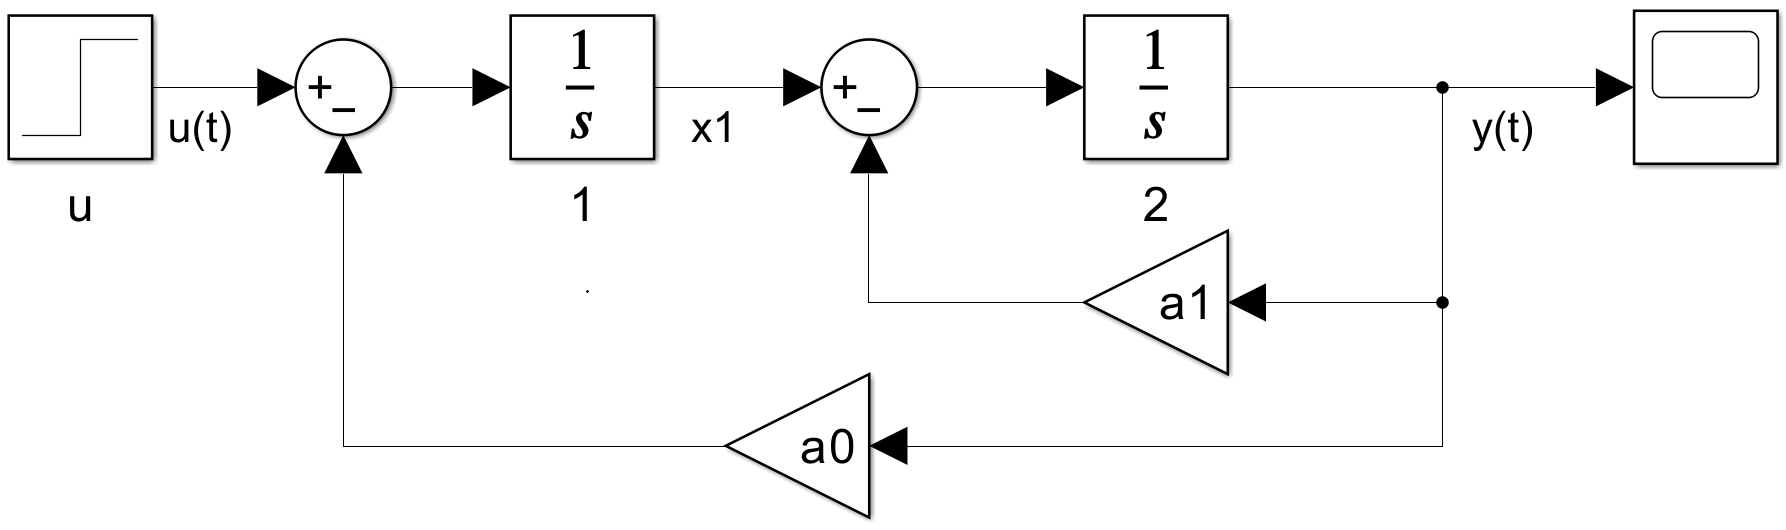
\includegraphics[width=\textwidth]{images/model1.png}
    \caption{Схема моделирования задания 1}
    \label{fig:1}
\end{figure}
Вычислим начальные данные интеграторов. На выходе интегратора 2 получаем $y(t)$, соответственно для него подставим $y_0$.
\newline
На выходе интегратора 1 получим $x_1$, причем:
\[
    \dot{y} = x_1 - a_1y
\]
Отсюда:
\[
    \dot{y}_0 = x_1(0) - a_1 y_0
\]
\[
    x_1(0) = \dot{y}_0 + a_1 y_0
\]
Теперь, можем построить графики моделирования исследуемых систем. В качестве входа $u(t)$ подставим $0$, чтобы получить свободное движение.
\newpage
\subsection{Результаты моделирования}
\begin{figure}[H]
    \centering
    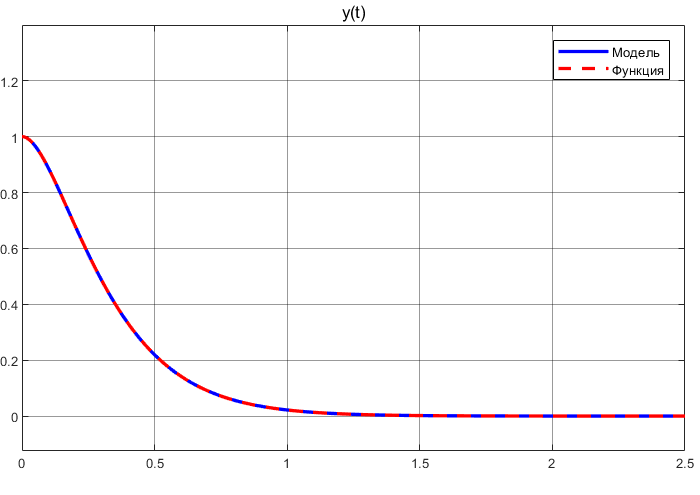
\includegraphics[width=0.8\textwidth]{images/t1f1.png}
    \caption{Эксперимент 1}
    \label{fig:2}
\end{figure}
\begin{figure}[H]
    \centering
    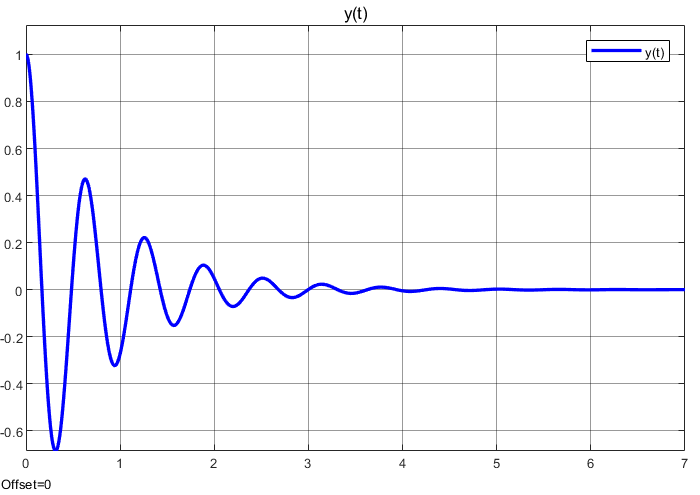
\includegraphics[width=0.8\textwidth]{images/t1f2.png}
    \caption{Эксперимент 2}
    \label{fig:2}
\end{figure}
\newpage
\begin{figure}[H]
    \centering
    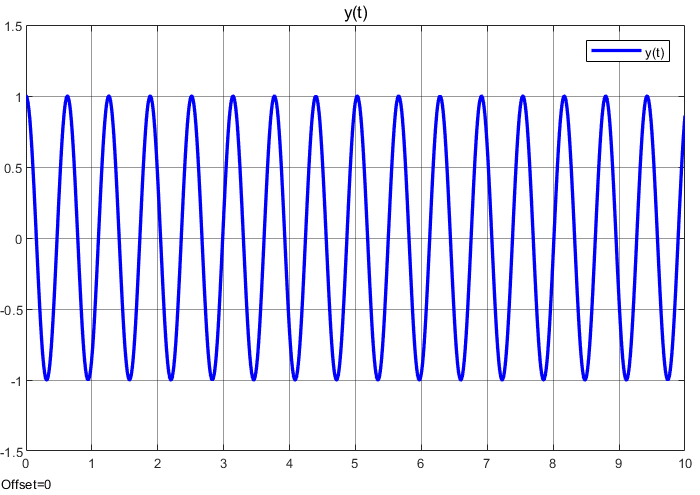
\includegraphics[width=0.8\textwidth]{images/t1f3.png}
    \caption{Эксперимент 3}
    \label{fig:2}
\end{figure}
\begin{figure}[H]
    \centering
    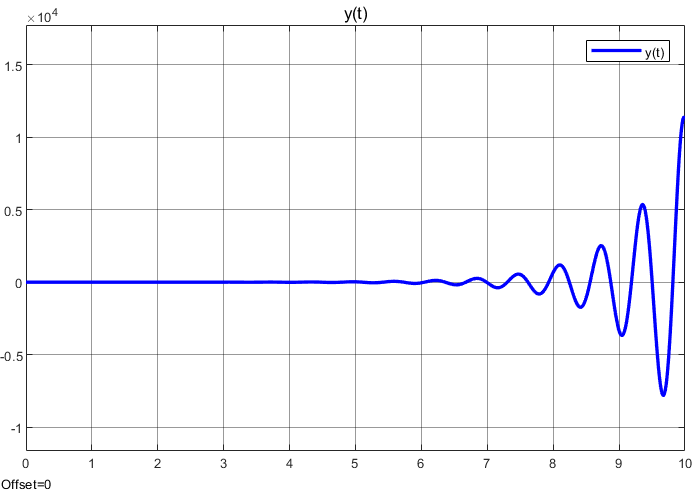
\includegraphics[width=0.8\textwidth]{images/t1f4.png}
    \caption{Эксперимент 4}
    \label{fig:2}
\end{figure}
\newpage
\begin{figure}[H]
    \centering
    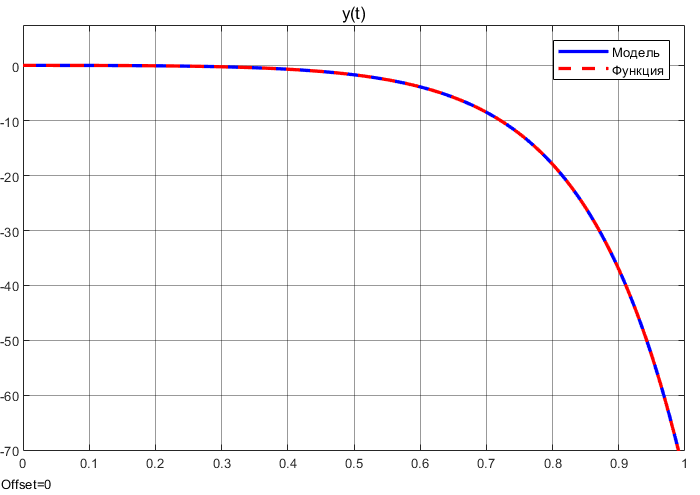
\includegraphics[width=0.8\textwidth]{images/t1f5.png}
    \caption{Эксперимент 5}
    \label{fig:2}
\end{figure}
\begin{figure}[H]
    \centering
    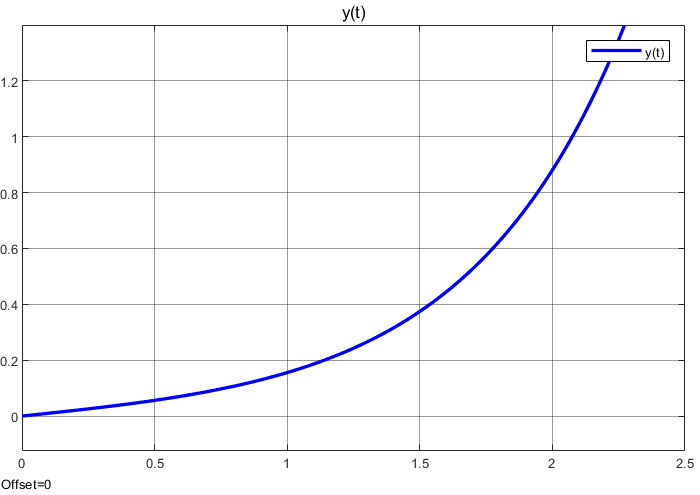
\includegraphics[width=0.8\textwidth]{images/t1f6.png}
    \caption{Эксперимент 6}
    \label{fig:2}
\end{figure}
\newpage
\subsection{Выводы по заданию 1}
Видим, что полученные при моделировании графики соответствуют полученным аналитически выражениям для свободных составляющих движения рассмотренных моделей. Для каждой из моделей хорошо виден ее тип сходимости, для моделей с комплексными корнями характеристического полинома видно наличие колебаний, а в моделях с действительными корнями колебания отсутствуют.
\newpage
\section{Задание 2}
\subsection{Схема моделирования Simulink для задания 2}
Вычислим параметры $T_1$ и $T_2$ из схемы в задании, так чтобы $\lambda_1$ и $\lambda_2$ были полюсами соответствующих передаточных функций.
\[
    T_1\lambda_1 + 1 = 0
\]
\[
    T_2\lambda_2 + 1 = 0
\]
\[
    T_1 = -\frac{1}{\lambda_1} = \frac{1}{5.5}
\]
\[
    T_2 = -\frac{1}{\lambda_2} = \frac{1}{6}
\]
Составим схему с соответствующими коэффициентами:
\begin{figure}[H]
    \centering
    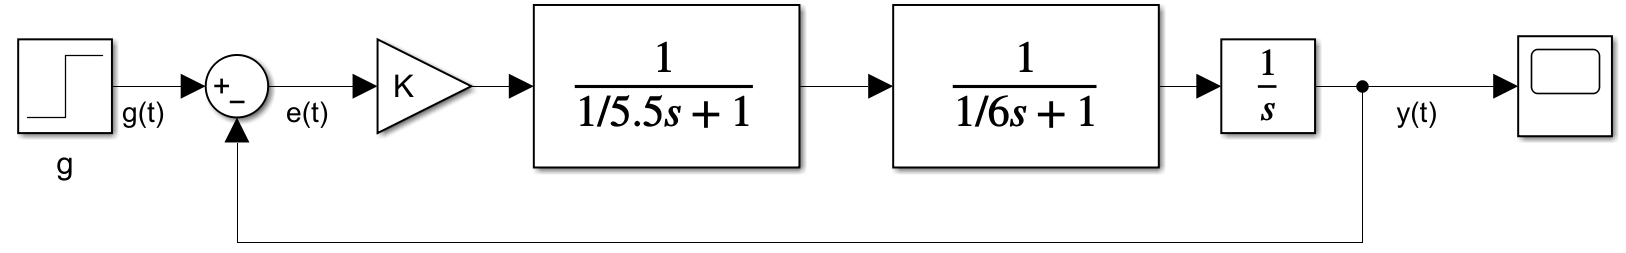
\includegraphics[width=\textwidth]{images/model2.png}
    \caption{Схема моделирования задания 2}
    \label{fig:1}
\end{figure}
\subsection{Определение области устойчивости системы}
Определим передаточную функцию смоделированной системы:
Представим четыре последовательных передаточных функции в схеме в виде одной передаточной функции $W_1(s)$:
\[
    W_1(s) = K \cdot \frac{1}{T_1 s + 1} \cdot \frac{1}{T_2 s + 1} \cdot \frac{1}{s}
\]
\[
    W_1(s) = \frac{K}{T_1 T_2 s^3 + (T_1 + T_2) s^2 + s}
\]
Таким образом можем представить схему этой модели как:
\begin{figure}[H]
    \centering
    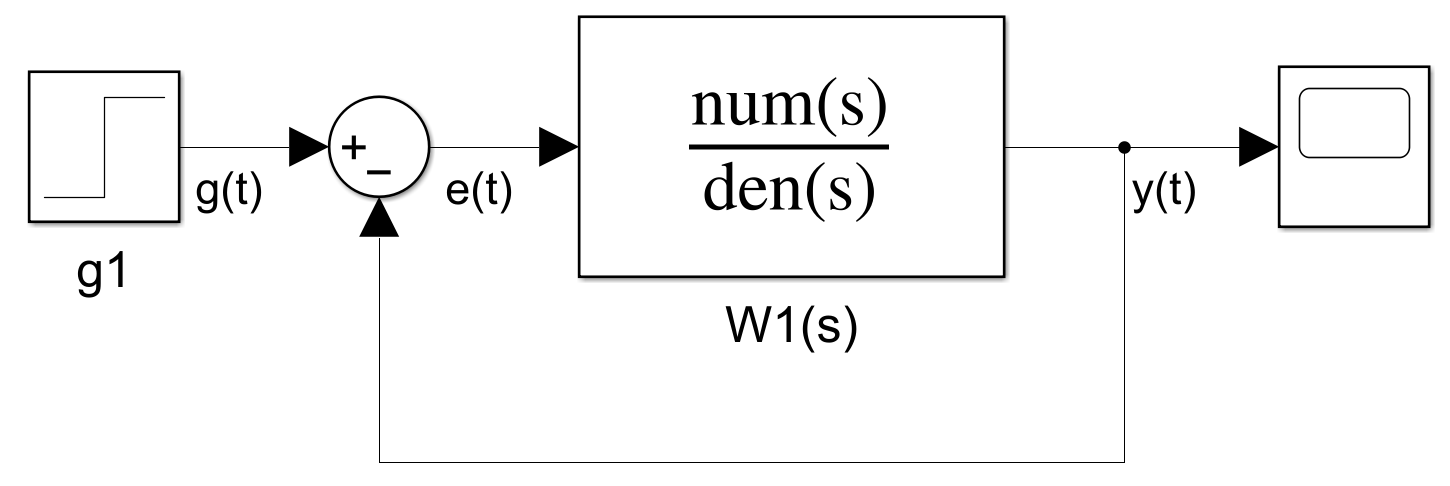
\includegraphics[width=0.8\textwidth]{images/model21.png}
    \caption{Схема после первого упрощения}
    \label{fig:1}
\end{figure}
\newpage
В таком случае передаточную функцию всей системы можно записать как:
\[
    W(s) = \frac{W_1(s)}{1 + W_1(s)} = \frac{\frac{K}{T_1 T_2 s^3 + (T_1 + T_2) s^2 + s}}{1 + \frac{K}{T_1 T_2 s^3 + (T_1 + T_2) s^2 + s}}
\]
\[
   W(s) = \frac{K}{T_1 T_2 s^3 + (T_1 + T_2) s^2 + s} / \frac{T_1 T_2 s^3 + (T_1 + T_2) s^2 + s + K}{T_1 T_2 s^3 + (T_1 + T_2) s^2 + s}
\]
\[
    W(s) = \frac{K}{T_1 T_2 s^3 + (T_1 + T_2) s^2 + s + K}
\]
Запишем матрицу Гурвица для полученного характеристического полинома:
\[
H = \begin{pmatrix}
    T_1 + T_2 & K & 0 \\
    T_1T_2 & 1 & 0 \\
    0 & T_1 + T_2 & K
\end{pmatrix}
\]
Найдем определители ее главных угловых миноров:
\[
    \Delta_1 = T_1 + T_2
\]
\[
    \Delta_2 = T_1 + T_2 - K T_1 T_2
\]
\[
    \Delta_3 = K (T_1 + T_2) - K^2 T_1 T_2 = K \Delta_2
\]
Зафиксируем $T_2 = \frac{1}{6}$.
\newline
Тогда, при $T_1 > 0$, $T_1 T_2 > 0$ следовательно, для выполнения критерия устойчивости Гурвица необходимо, чтобы все определители были положительны:
\[
    \Delta_1 = T_1 + \frac{1}{6} > 0, \ \ \text{так как} \ \ T_1 > 0
\]
\[
    \Delta_2 = T_1 + \frac{1}{6} - \frac{K}{6} T_1 > 0 \ \ <=> \ \ 6 + \frac{1}{T_1} > K, \ \ \text{при} \ \ T_1 > 0
\]
\[
    \Delta_3 = K \Delta_2 > 0,  \ \ \Delta_2 > 0 \ \ <=> \ \ K > 0
\]
Также рассмотрим $T_1 < 0$, тогда $T_1 T_2 < 0$. Домножим характеристический полином на $-1$, тогда новый старший коэффициент будет положителен, знаки определителей всех угловых миноров нечетного размера будут противоположны по знаку определителям соответствующих миноров исходной матрицы Гурвица, а определители миноров четного размера в старой и новой матрице Гурвица будут равны. Исходя из этого запишем новые ограничения:
\[
    \Delta_{1new} = -T_1 - \frac{1}{6} > 0 \ \ <=> \ \ T_1 < -\frac{1}{6}
\]
\[
    \Delta_{2new} = \Delta_{2} > 0 \ \ <=> \ \ 6 + \frac{1}{T_1} < K, \ \ \text{при} \ \ T_1 > 0
\]
\[
    \Delta_{3} = -K \Delta_2 > 0, \ \ \Delta_2 > 0 \ \ <=> \ \ K < 0 
\]
\newpage
Таким образом, можем составить систему неравенств соответствующую выполнению критерия Гурвица:
\[
    \left[
        \begin{gathered}
            \left\{
                \begin{aligned}
                    T_1 > 0 \\
                    K > 0 \\
                    6 + \frac{1}{T_1} > K
                \end{aligned}
            \right.
            \\
            \left\{
                \begin{aligned}
                    T_1 < \frac{-1}{6} \\
                    K < 0 \\
                    6 + \frac{1}{T_1} < K
                \end{aligned}
            \right.
        \end{gathered}
    \right.
\]
Также отдельно опишем условия при которых $a_0$ или один из миноров матрицы Гурвица строго равен $0$:
\[
    a_0 = \frac{T_1}{6} = 0 \ \ <=> \ \ T_1 = 0
\]
\[
    \Delta_1 = T_1 + \frac{1}{6} = 0 \ \ <=> \ \ T_1 = -\frac{1}{6}
\]
\[
    \Delta_2 = T_1 + \frac{1}{6} - \frac{K}{6} T_1 = 0 \ \ <=> \ \ 6 + \frac{1}{T_1} = K
\]
\[
    \Delta_3 = K\Delta_2 = 0 \ \ <=> \ \ K = 0 \ \ \text{или} \ \ \Delta_2 = 0
\]
Построим график этой системы в Desmos, при этом область устойчивости выделим синим цветом, границы с условием равенства $a_0$ или одного из миноров матрицы Гурвица нулю выделим красным:
\begin{figure}[H]
    \centering
    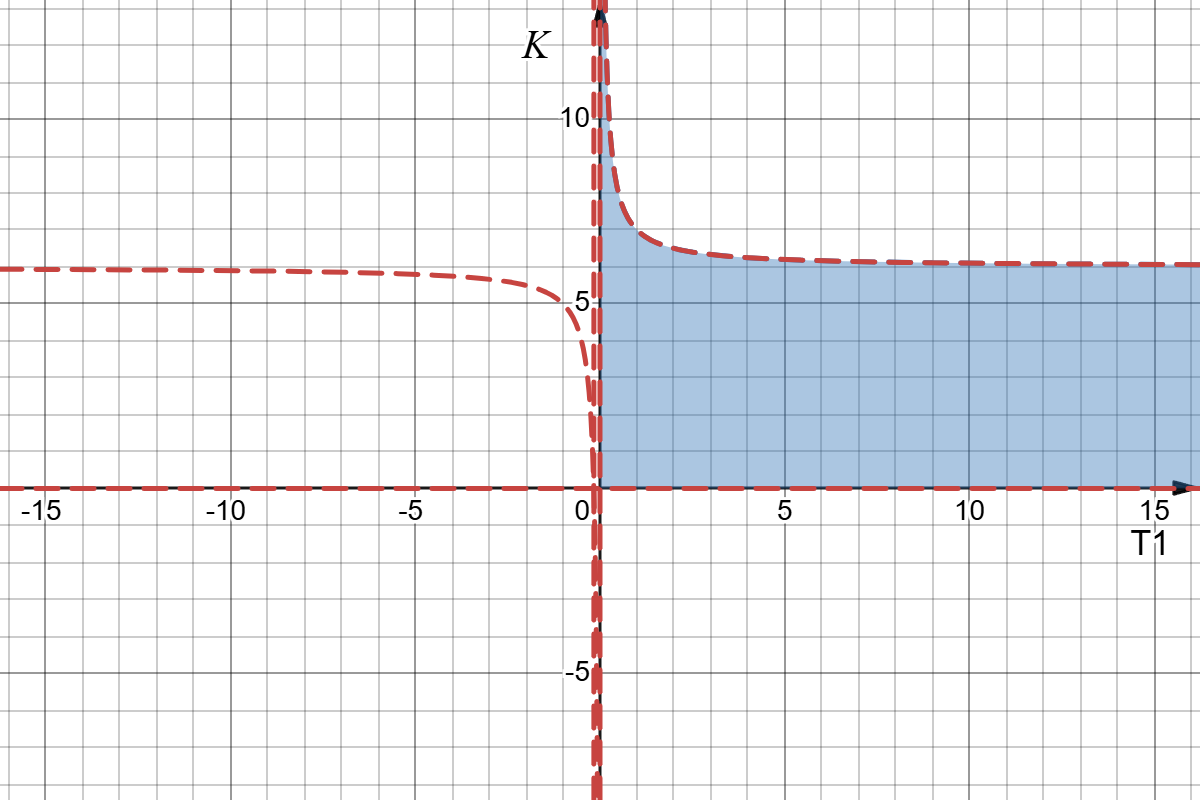
\includegraphics[width=0.8\textwidth]{images/OblUst.png}
    \caption{График области устойчивости (синий) и граничных условий (красный)}
    \label{fig:1}
\end{figure}
Можем заметить, что не все точки граничных линий лежат на границе области устойчивости, так как характеристический полином может иметь мнимый корень при наличии корней с положительной действительной частью.
\newpage
\subsection{Моделирование системы в различных состояних устойчивости}
Получив ограничения на область устойчивости рассмотрим графики моделирования, выбирая параметры $T_1, T_2$ и $K$ соответствующие области устойчивости, на границе устойчивости, неустойчивой системе. При этом перестроим схему моделирования в форму вход-выход:
\[
    W(s) =  W(s) = \frac{K}{T_1 T_2 s^3 + (T_1 + T_2) s^2 + s + K} = \frac{\frac{K}{T_1 T_2}}{s^3 + \frac{T_1 + T_2}{T_1 T_2}s^2 + \frac{1}{T_1 T_2}s + \frac{K}{T_1 T_2}}
\]
\begin{figure}[H]
    \centering
    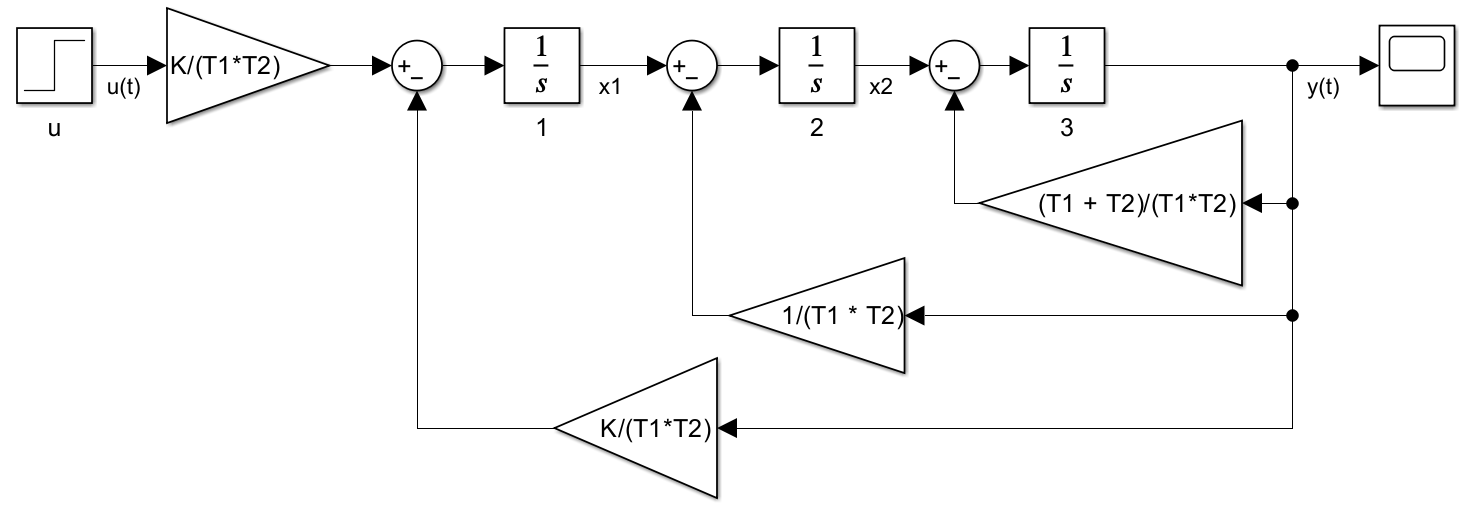
\includegraphics[width=\textwidth]{images/model2f.png}
    \caption{Схема в форме вход-выход}
    \label{fig:1}
\end{figure}
Для этого приведем в соответствие начальные данные для $y(t)$ ($y(0) = 1$, $\dot{y}(0) = 0$, $\ddot{y}(0) = 0$)
\newline
Начальные данные для третьего интегратора равны $y(0) = 1$
\newline
Для выхода второго интегратора:
\[
    \dot{y} = x_2 - \frac{T_1+T_2}{T_1 T_2}y
\]
\[
    x_2(0) = \dot{y}(0) + \frac{T_1+T_2}{T_1 T_2}y(0) = \frac{T_1+T_2}{T_1 T_2}
\]
Для первого интегратора:
\[
    \dot{x_2} = x_1 - \frac{1}{T_1 T_2}y
\]
С другой стороны:
\[
    \dot{x_2} = \ddot{y}(0) + \frac{T_1+T_2}{T_1 T_2}\dot{y}(0) = 0, \ \ \text{при} \ \ t = 0
\]
Отсюда:
\[
    x_1(0) = \frac{1}{T_1 T_2}
\]

\newpage
\subsection{Результаты моделирования в задании 2}
Зная область устойчивости и параметры моделирования построим графики моделирования систем с разными наборами параметров $T_1, T_2, K$.
\newline
В качестве таких наборов возьмем:
\newline
\begin{itemize}
    \item $K = 2, T_1 = 2, T_2 = \frac{1}{6}$ - область устойчивости; \\
    \item $K = 10, T_1 = \frac{1}{4}, T_2 = \frac{1}{6}$ граница устойчивости \\
    \item $K = 5, T_1 = 10, T_2 = \frac{1}{6}$ неустойчивая система
\end{itemize}
При этом для моделирования свободного движения вход $u(t)$ считаем равным $0$.
\begin{figure}[H]
    \centering
    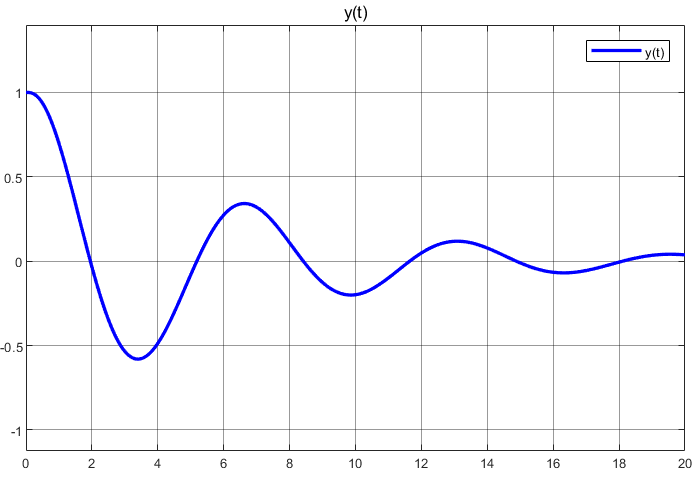
\includegraphics[width=0.8\textwidth]{images/t2f1.png}
    \caption{$K = 2, T_1 = 2, T_2 = \frac{1}{6}$ область устойчивости}
    \label{fig:2}
\end{figure}
\newpage
\begin{figure}[H]
    \centering
    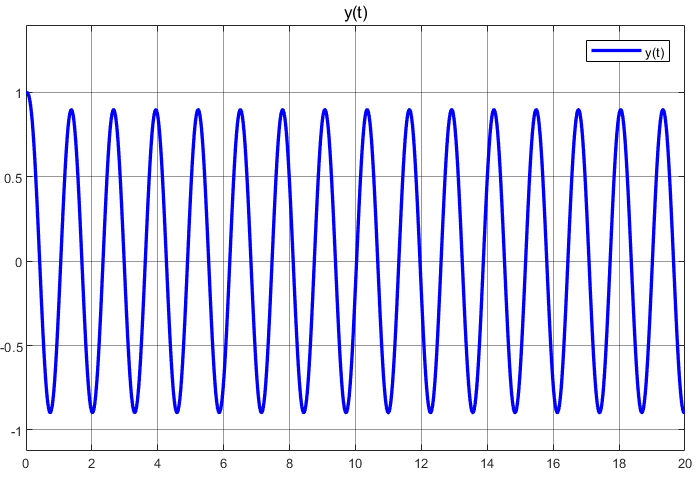
\includegraphics[width=0.8\textwidth]{images/t2f2.png}
    \caption{$K = 10, T_1 = \frac{1}{4}, T_2 = \frac{1}{6}$ граница устойчивости}
    \label{fig:2}
\end{figure}
\begin{figure}[H]
    \centering
    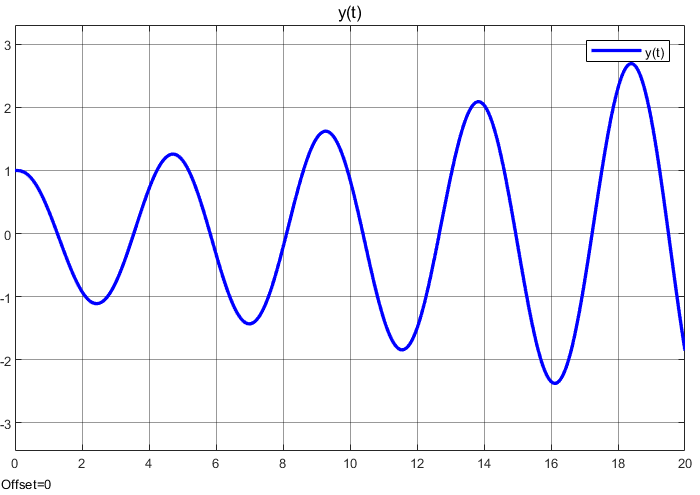
\includegraphics[width=0.8\textwidth]{images/t2f3.png}
    \caption{$K = 5, T_1 = 10, T_2 = \frac{1}{6}$ неустойчивая система}
    \label{fig:2}
\end{figure}
\newpage
\subsection{Выводы по заданию 2}
В результате вычисления области устойчивости системы методом Гурвица удалось заметить, что граница области устойчивости является подмножеством области в которой $a_0$ или определитель одного из миноров равен $0$.
\newline
При моделировании же на практике систем с различными параметрами $T_1, T_2, K$ мы получили тот тип устойчивости, который следует из теоретических выкладок.
\newpage
\section{Задание 3}
Будем строить командный генератор с желаемым выходом:
\[
    g_{\textit{ж}} (t) = 3e^{-3t} \sin{(2t)} + 1.5 \sin{(5t)}
\]
Заметим, что сигнал представляет собой сумму двух мод. Первая мода - произведение экспоненты с показателем $-3t$ и синуса с частотой $2$, вторая мода - синус с частотой $5$ без экспоненты. Таким образом, характеристический полином искомой системы управления имеет две пары комплексно сопряженных корней: $-3 \pm 2i$ и $\pm 5i$.
\newline
Теперь попробуем воспользоваться методом Жорданова представления. Составим матрицу $G$ из двух Жордановых клеток для этих пар корней:
\[
    G = \begin{pmatrix}
        -3 & 2 & 0 & 0 \\
        -2 & -3 & 0 & 0 \\
        0 & 0 & 0 & 5 \\
        0 & 0 & -5 & 0 \\
    \end{pmatrix}
\]
Запишем выражение для выхода командного генератора:
\[
    g(t) = H \cdot e^{Gt} \cdot z(0)
\]
Выразим матричную экспоненту для полученной Жордановой матрицы $G$:
\[
    e^{Gt} = \begin{pmatrix}
        e^{-3t}\cos{(2t)} & e^{-3t}\sin{(2t)} & 0 & 0 \\
        -e^{-3t}\sin{(2t)} & e^{-3t}\cos{(2t)} & 0 & 0 \\
        0 & 0 & \cos{(5t)} & \sin{(5t)} \\
        0 & 0 & -\sin{(5t)} & \cos{(5t)} \\
    \end{pmatrix}
\]
Теперь перепишем выражение для выхода генератора подставив в него матричную экспоненту:
\[
    g(t) = \begin{pmatrix}
        h_1 & h_2 & h_3 & h_4 \\
    \end{pmatrix} \cdot \begin{pmatrix}
        e^{-3t}\cos{(2t)} & e^{-3t}\sin{(2t)} & 0 & 0 \\
        -e^{-3t}\sin{(2t)} & e^{-3t}\cos{(2t)} & 0 & 0 \\
        0 & 0 & \cos{(5t)} & \sin{(5t)} \\
        0 & 0 & -\sin{(5t)} & \cos{(5t)} \\
    \end{pmatrix} \cdot \begin{pmatrix}
        z_1(0) \\
        z_2(0) \\
        z_3(0) \\
        z_4(0) \\
    \end{pmatrix}
\]
\[
    g(t) = z_1(0) \cdot (h_1e^{-3t}\cos{(2t)} - h_2e^{-3t}\sin{(2t)}) + z_2(0) \cdot (h_1e^{-3t}\sin{(2t)} + h_2e^{-3t}\cos{(2t)}) + 
\]
\[
    + z_3(0) \cdot (h_3\cos{(5t)} - h_4\sin{(5t)}) + z_4(0) \cdot (h_3\sin{(5t)} + h_4\cos{(5t)})
\]
Вынесем гармоники за скобки:
\[
    g(t) = e^{-3t}\cos{(2t)} \cdot (z_1(0)h_1 + z_2(0)h_2) + e^{-3t}\sin{(2t)} \cdot (-z_1(0)h_2 + z_2(0)h_1) +
\]
\[
    + \cos(5t) \cdot (z_3(0)h_3 + z_4(0)h_4) + \sin{(5t)} \cdot (-z_3(0)h_4 + z_4(0)h_3)
\]
\newpage
Отсюда можем составить систему уравнений, так как коэффициенты перед гармониками в искомой функции известны:
\[
    \left\{
        \begin{aligned}
            z_1(0)h_1 + z_2(0)h_2 = 0 \\
            -z_1(0)h_2 + z_2(0)h_1 = 3 \\
            z_3(0)h_3 + z_4(0)h_4 = 0 \\
            -z_3(0)h_4 + z_4(0)h_3 = 1.5
        \end{aligned}
    \right.
\]
Найдем произвольное решение полученной системы уравнений. Пусть $h_1 = 1$, $h_2 = 0$, $h_3 = 1$, $h_4 = 0$; тогда:
\[
    \left\{
        \begin{aligned}
            z_1(0) = 0 \\
            z_2(0) = 3 \\
            z_3(0) = 0 \\
            z_4(0) = 1.5
        \end{aligned}
    \right.
\]
Получили матрицы $G$, $H$, $z(0)$, а, следовательно представили командный генератор:
\[
    G = \begin{pmatrix}
        -3 & 2 & 0 & 0 \\
        -2 & -3 & 0 & 0 \\
        0 & 0 & 0 & 5 \\
        0 & 0 & -5 & 0 \\
    \end{pmatrix}
\]
\[
    H = \begin{pmatrix}
        1 & 0 & 1 & 0 \\
    \end{pmatrix}
\]
\[
    z(0) = \begin{pmatrix}
        0 \\
        3 \\
        0 \\
        1.5 \\
    \end{pmatrix}
\]
\[
    g(t) = H \cdot e^{Gt} \cdot z(0)
\]
\subsection{Моделирование командного генератора в Simulink}
Представим командный генератор моделью в пространстве состояний:
\[
    \left\{
        \begin{aligned}
            \dot{z} = Gz \\
            g = Hz
        \end{aligned}
    \right.
\]
\[
    \left\{
        \begin{aligned}
            \begin{pmatrix}
            \dot{z_1} \\
            \dot{z_2} \\
            \dot{z_3} \\
            \dot{z_4} \\
    \end{pmatrix} = \begin{pmatrix}
        -3 & 2 & 0 & 0 \\
        -2 & -3 & 0 & 0 \\
        0 & 0 & 0 & 5 \\
        0 & 0 & -5 & 0 \\
    \end{pmatrix} \cdot \begin{pmatrix}
            z_1 \\
            z_2 \\
            z_3 \\
            z_4 \\
    \end{pmatrix} \\
        g = \begin{pmatrix}
        1 & 0 & 1 & 0 \\
    \end{pmatrix} \cdot \begin{pmatrix}
            z_1 \\
            z_2 \\
            z_3 \\
            z_4 \\
    \end{pmatrix}
        \end{aligned}
    \right.
\]
\newpage
Перепишем систему из матричного вида в обыкновенный:
\[
    \left\{
        \begin{aligned}
            \dot{z_1} = -3z_1 + 2z_2 \\
            \dot{z_2} = -2z_1 - 3z_2 \\
            \dot{z_3} = 5z_4 \\
            \dot{z_4} = -5z_3 \\
            g = z_1 + z_3
        \end{aligned}
    \right.
\]
На основе полученной системы уравнений составим схему моделирования:
\begin{figure}[H]
    \centering
    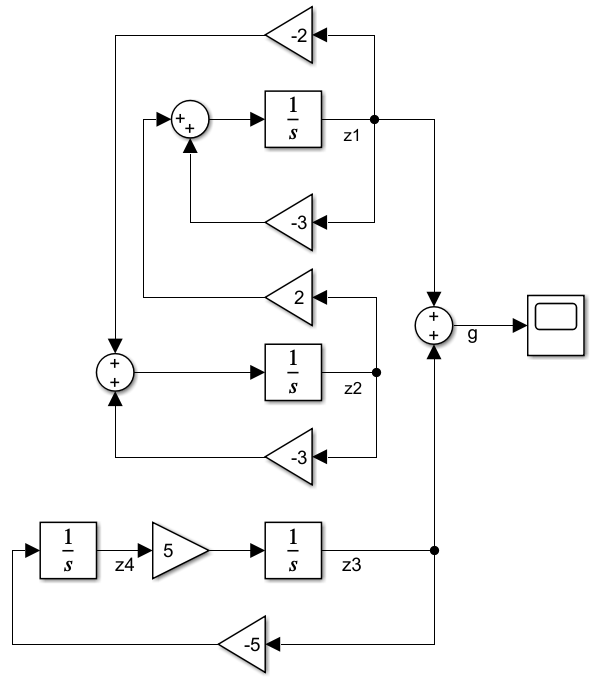
\includegraphics[width=0.8\textwidth]{images/model3.png}
    \caption{Схема моделирования командного генератора в Simulimk}
    \label{fig:1}
\end{figure}
В качестве начальных значений интеграторов подставим соответствующие координаты вектора $z(0)$.
\newpage
С помощью полученной модели построим график выхода генератора. Также построим в тех же осях график функции $g_{\textit{ж}}(t)$ и сравним полученные графики.
\begin{figure}[H]
    \centering
    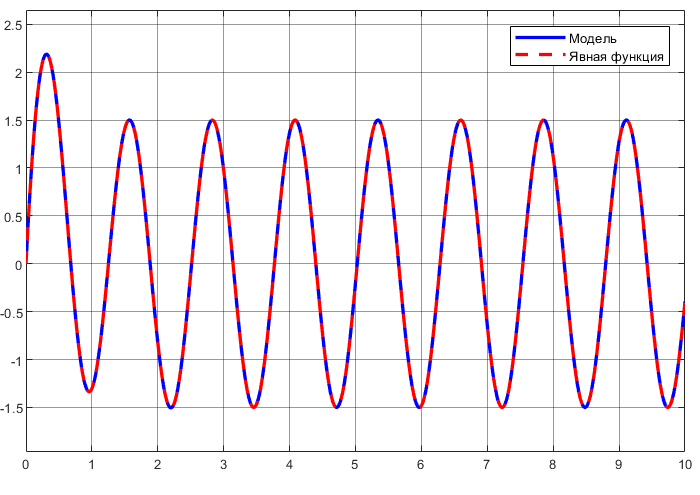
\includegraphics[width=0.8\textwidth]{images/t3f1.png}
    \caption{Сравнение графика функции и графика модели генератора}
    \label{fig:2}
\end{figure}
Также на каждом шаге вычислим ошибку $e(t)$ как $g_{\textit{ж}}(t) - g(t)$ и построим ее график:
\begin{figure}[H]
    \centering
    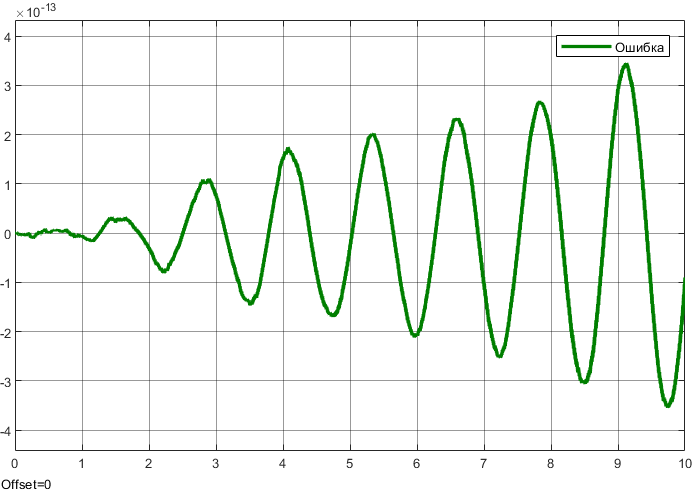
\includegraphics[width=0.8\textwidth]{images/t3f2.png}
    \caption{График разности явной функции и модели генератора}
    \label{fig:2}
\end{figure}
\newpage
\subsection{Выводы по 3 заданию}
В результате выполнения задания рассчет матмодели командного генератора с помощью метода Жордана оказался успешен. График модели simulink, построенной на основе полученной математической модели, достаточно точно совпал с графиком явно рассчитанной функции $g_{\textit{ж}}(t)$. Их разность при этом постепенно возрастает по модулю с течением времени, но очень мала на протяжении всего времени моделирования (порядка $10^{-13}$)
\section{Выводы по лабораторной работе}
В данной лабораторной работе мы провели вычисление свободной составляющей движения для набора линейных систем управления второго порядка и построили соотвествующие графики с помощью модели в Simulink.
\newline
Далее мы вычислили область устойчивости линейной системы третьего порядка в зависимости от ее параметров и построили графики свободной составляющей движения для наборов параметров, соответствующих разным видам устойчивости.
\newline
Далее было проведен расчет командного генератора по заданной целевой функции. Можно заметить, что полученный командный генератор также является свободной составляющей движения для некоторой системы управления в форме вход-состояние-выход.
\end{document}

